%\section{Understanding and Modeling Transient Server Preemptions}
%\section{Modeling the Dynamics of Transient Server Preemptions}
%\section{Preemption Dynamics of Transient Cloud Servers}
\vspace*{\subsecspace}
\section{Modeling Preemption Dynamics}
\label{sec:preemption-dynamics}

%Understanding the nature and dynamics of transient cloud servers such as their preemption frequency is a prerequisite to understand and improve the performance of applications.

\eat{In order to understand and improve the performance of applications running on transient cloud servers, we must understand the nature and dynamics of their preemptions.
The preemption characteristics are governed by the supply of surplus resources, the demand for cloud resources, and the resource allocation policies enforced by the cloud operator.
Therefore, in this section, we present empirical and analytical models to help us understand the nature of preemptions. 
}

To measure and improve the performance of applications running on transient cloud servers, it is critical to understand the nature and dynamics of their preemptions.
The preemption characteristics are governed by the supply of surplus resources, the demand for cloud resources, and the resource allocation policies enforced by the cloud operator.
In this section, we present empirical and analytical models that describe these characteristics and enable an intuitive understanding of the nature of preemptions. 


% Transient cloud servers, by their very nature have limited availability and are frequently preempted.
% These preemptions are akin to fail-stop failures, and are often preceeded by a small advance warning (few seconds) to allow for graceful shutdowns.

% Since preemptions can impact the availability, performance, and cost of running applications, in this section, we examine their preemption characteristics.
% This modeling is important, because having a model of the availability can be useful in the context of predicting the running times of applications.
% Cloud providers offer a large number of servers of different configurations and types.
% Since transient server availability is fundamentally tied to supply and demand, the availability of servers of different types can be significantly different. 
% Thus, selecting the ``right'' server type is crucial for minimizing the overall costs. 



\vspace*{\subsecspace}
\subsection{The Need For Empirical Preemption Models}
\label{subsec:need-for-empirical}

Amazon's EC2 spot instances were the original transient cloud servers.
The preemptions of EC2 spot instances are based on their \emph{price}, which is dynamically adjusted based on the supply and demand of cloud resources.
Spot prices are based on a continuous second-price auction, and if the spot price increases above a pre-specified maximum-price, then the server is preempted~\cite{spot-pricing2}.

Thus, the time-series of these spot prices can be used for understanding preemption characteristics such as the frequency of preemptions and the ``Mean Time To Failure'' (MTTF) of the spot instances. 
Publicly available\footnotemark historical spot prices can be used to characterize and model spot instance preemptions~\cite{spotcheck,bid-cloud}. %Add lots more here 
For example, past work has analyzed spot prices and shown that the MTTFs of spot instances of different hardware configurations and geographical zones range from a few hours to a few days~\cite{prateek-thesis, wolski_probabilistic_2017, icdcs-spotlight}. 


\footnotetext{Amazon posts Spot prices of 3 months, and researchers have been collecting these prices since 2010~\cite{bidding4}.}

However, Amazon has recently changed the preemption characteristics of spot instances, and servers are now preempted even if the spot price is below the maximum price~\cite{spotweb, bid-change}.
Thus, spot prices are no longer a completely reliable indicator of preemptions, and preemptions can no longer be inferred from looking at prices alone.
Therefore, new techniques are required to model preemption dynamics that can supplement the earlier price-based approaches, and we develop these techniques next.

%\cite{alicloud-spot, packet-spot}

%\subsection{Empirical model of preemptions}
%\subsection{Empirical preemption behavior}
\vspace*{\subsecspace}
\subsection{Empirical Study Of Preemptions In Google Cloud}

The preemptions of transient servers need not be related to their price.
For example, Google's Preemptible VMs and Azure Batch VMs have a \emph{fixed} price relative to their non-preemptible counterparts. 
In such cases, price-based models are inadequate, and other approaches to understand preemptions are required.

This task is further complicated by the fact that these cloud operators (Google and Microsoft) do not currently provide any information about preemption characteristics. 
Thus, relatively little is known about the preemptions (and hence the performance) of these transient VMs. %significantly limiting their use?
%
To understand preemption dynamics of transient servers, we conduct a large-scale empirical measurement study which is the first of its kind. 
We launched more than 1,500 Google Preemptible VMs of different types over a two month period (Feb--April 2019), and measured their time to preemption (i.e., their useful lifetime).\footnotemark

\footnotetext{We will release the complete preemption dataset and hope that other researchers can benefit.} %Weaksauce 


\begin{figure}
  \centering
  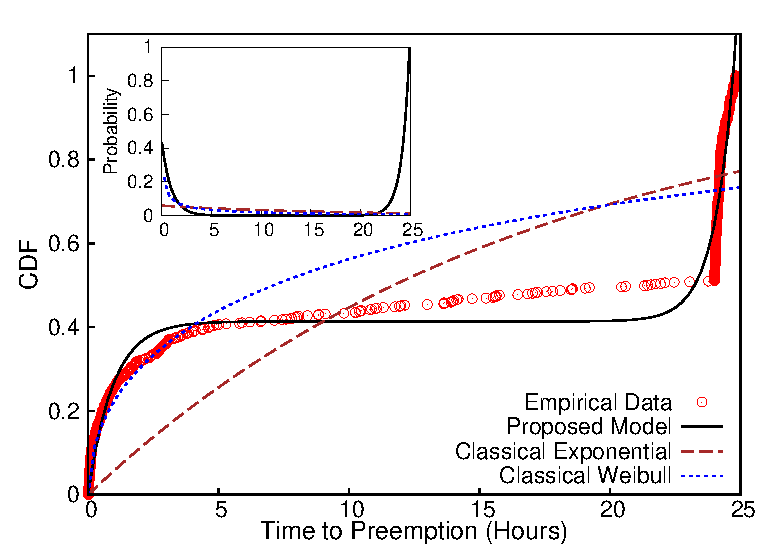
\includegraphics[width=0.4\textwidth]{../graphs/scispot-fig-cdf-prob-inset-time.eps}
  \caption{CDF of lifetimes of Google Preemptible VMs. Our proposed distribution for modeling the constrained preemption dynamics provides better fits to the empirical data compared to the conventional exponential and the Weibull distributions. Inset shows the probability of failure as a function of time for the three distributions.}
  \label{fig:gcp1}
\end{figure}

A sample of over 100 such preemption events are shown in Figure~\ref{fig:gcp1}, which shows cumulative distribution function (CDF) of the VM lifetimes of the \texttt{n1-highcpu-16} VM in the \texttt{us-east1-b} zone. 
%enter the type of VM for which the data is shown
Note that the cloud operator (Google) caps the \emph{maximum} lifetime of the VM to 24 hours, and all the VMs are preempted before that limit. 
Furthermore, the lifetimes of VMs are \emph{not} uniformly distributed, but have three distinct phases. 
In the first (initial) phase, characterized by VM lifetime $t\in [0, 3]$ hours, we observe that many VMs are quickly preempted after they are launched, and thus have a steep rate of failure (derivative of the CDF) initially.
%; the rate of failure or preemptions can be obtained by taking the derivative of the CDF. 
In the second phase, VMs that survive past 3 hours enjoy a relatively low preemption rate over a relatively broad range of lifetime (characterized by the slowly rising CDF in Figure~\ref{fig:gcp1}). The third and final phase exhibits a steep increase in the number of preemptions as the preemption deadline of 24 hours approaches. The overall rate of preemptions is ``bathtub'' shaped as shown in the inset of Figure~\ref{fig:gcp1}.
%\it I think we should show the probability plot to exhibit the bath tub shape

%The preemption rate is ``bath tub'' shaped, with VMs that survive past 3 hours enjoying a relatively low preemption rate, and finally a steep increase in the number of preemptions as the preemption deadline (24 hours) approaches. 

We note that this preemption behavior, imposed by the constraint of the small 24 hour  lifetime, is \emph{substantially} different from conventional failure characteristics of hardware components and even EC2 spot instances.
In these ``classical'' setups, the rate of failure  usually follows an exponential distribution $f(t) = \lambda e^{-\lambda t}$, where $\lambda=1/\text{MTTF}$.
Figure~\ref{fig:gcp1} shows the CDF ($=1-e^{-\lambda t}$) of the exponential distribution when fitted to the observed preemption data, by finding the distribution parameter $\lambda$ that minimizes the least squares error.
The classic exponential distribution is unable to model the observed preemption behavior because it assumes that the rate of preemptions is independent of the lifetime of the VMs, i.e., the preemptions are \emph{memoryless}.
%The primary reason is that the exponential distribution assumes that the \vj{the rate of preemptions is independent of the lifetime of the VMs} (preemptions are \emph{memoryless}), which does not hold true when there is a fixed upper bound on the lifetime, as is the case for Google Preemptible VMs. \vj{In other words, the conventional approach is insufficient to model constrained preemption dynamics.}
%We attribute this deficiency to the central assumption made in the underlying reliability theory principles that leads to the classical exponential distribution: the rate of preemptions is independent of the lifetime of the VMs, in other words, the preemptions are \emph{memoryless}.
This assumption breaks down when there is a fixed upper bound on the lifetime, as is the case for Google Preemptible VMs, and the conventional approach becomes insufficient to model this constrained preemption dynamics. 

\vspace*{\subsecspace}
\subsection{Model Of Constrained Preemption Dynamics}
\label{subsec:analytical-model}

We now develop an analytical model for preemption dynamics that is faithful to the empirically observed data and provides a basis for developing running-time and cost-minimizing optimizations. % presented in Section~\ref{sec:design}. 
%
To describe failures (preemptions) that are not memoryless (i.e., increasing or decreasing failure rate over time), the classic Weibull distribution with CDF $F(t)=1-e^{-(\lambda t)^k}$ is often employed. However, we find that the Weibull distribution is also unable to fit the empirical data (Figure~\ref{fig:gcp1}). 

The non-trivial bathtub-shaped failure rate of Google preemptible VMs (Figure~\ref{fig:gcp1}) requires models that capture the sudden onset of  the rise in preemptions near the deadline. 
%which imposes a dynamics that is more akin to a constrained dynamics problem as opposed to dynamics characterized with a gradually rising failure rate.
Our new model, informed by the cumulative distribution of lifetimes that has multiple distinct temporal phases, addresses this need. The key assumption underlying our model is the presence of two distinct failure processes.
%that give rise to a new probability distribution characterizing the preemptions and the observed CDF, and ensure the dependence of the rate of failure on the VM lifetime. 
The first process dominates over the initial temporal phase and yields the classic exponential distribution that captures the high rate of early preemptions. The second process dominates over the final phase near the 24 hour maximum VM lifetime and is assumed to be characterized by an exponential term that captures the sharp rise in preemptions that results from this constrained lifetime. 
%Generally, these two processes jointly determine the dynamics of preemptions during the middle phase where a relatively constant or a slowly rising number of preemptions with time is observed.
%; in practice, based on the fits to the empirical data, we observe the first process to dominate over the second during this phase as well. 

%The first two phases are reasonably captured by the classic exponential distribution. In order to model the overall observed empirical CDF, we add another term that captures the failure process near the 24 hour maximum VM lifetime,  and construct a \emph{new} probability distribution. 
%
%we develop a \emph{new} probability distribution that is composed by blending two failure processes that act on different temporal phases over the 24 hour maximum lifetime of the VMs. 
%
%We write the general form of our blended preemption CDF as follows:

Based on these observations, we propose the following general form for the CDF:
\begin{equation}
  \label{eq:blend1}
  \mathscr{F}\left(t\right) = A\left(1-e^{-\frac{t}{\tau_1}} + e^{\frac{t-b}{\tau_2}}\right),
\end{equation}
where $t$ is the time to preemption, $1/\tau_1$ is the rate of preemptions in the initial phase, $1/\tau_2$ is the rate of preemptions in the final phase, $b$ denotes the time that characterizes ``activation'' of the final phase where preemptions occur at a very high rate, and $A$ is a scaling constant.
In practice, typical fit values yield $b \approx 24$ hours, and $\tau_2 \approx 1$ hour, which ensures that our proposed distribution meets the initial condition $\mathscr{F}(0) \approx 0$.

%of  0 $\approx 0$ premptions.
%used to scale the CDF to ensure that the initial conditions ($F(0)=0$) are met.

For most of its life, a VM sees failures according to the classic exponential distribution with a rate of failure equal to $1/\tau_1$ -- this behavior is captured by the $1-e^{-t/\tau_1}$ term in Equation~\ref{eq:blend1}. 
%However, this does not capture the finite lifetime of the VM imposed by the cloud operator.
As VMs get closer to their maximum lifetime imposed by the cloud operator, they are reclaimed (i.e., preempted) at a high rate $1/\tau_2$, which is captured by the second exponential term, $e^{(t-b)/\tau_2}$ of Equation~\ref{eq:blend1}. 
Shifting the argument ($t$) of this term by $b$ ensures that the exponential reclamation is only applicable near the end of the VM's maximum lifetime and does not dominate over the entire temporal range. 
%As noted before, $1/\tau_2$ is the rate of this reclamation. 

The analytical model and the associated  distribution function $\mathscr{F}$ introduced above provides a much better fit to the empirical data (Figure~\ref{fig:gcp1}) and captures the different phases of the preemption dynamics through parameters $\tau_1, \tau_2, b$, and $A$. These parameters can be obtained for a given empirical CDF using least squares function fitting methods.

%\footnotemark 
%
%\footnotetext{More details about the distribution fitting are presented in the implementation section(~\ref{sec:impl}}
%

Further, the failure or preemption rate can be derived from this CDF as:
\begin{equation}
\label{eq:failrate}
p(t) = \dfrac{d \mathscr{F}(t)} {dt} = A \left(\dfrac{1}{\tau_1}e^{-t/\tau_1} + \dfrac{1}{\tau_2}e^{\frac{t-b}{\tau_2}}\right).
\end{equation}
$p(t)$ vs. $t$ yields a bathtub type failure rate function for the associated fit parameters (inset of Figure~\ref{fig:gcp1}).
In the next section, we use this analytical model for optimizing cloud resource selection to run scientific computing applications at low cost and shorter running (turnaround) times.

In the absence of any prior work on constrained preemption dynamics, our motivation is to develop an interpretable model with a minimal number of parameters, that provides a sufficiently accurate characterization of observed preemptions data. 
As is evident from Figure~\ref{fig:gcp1}, our model shows deviations from the data near the halfway point within the 24 hour lifetime. 
Further generalization of this model to include more failure processes would introduce more parameters and reduce the generalization power.
Exploring other approaches of modeling bathtub-type failure rates (e.g., exponential Weibull distributions) \cite{mudholkar1993exponentiated,crevecoeur1993model} is part of our future work. 


\eat{
We emphasize that our motivation is to develop an interpretable \emph{minimal} model that provides a sufficiently accurate description of the observed constrained preemption dynamics of Google VMs with a minimal number of meaningful parameters. 
As is evident from Figure~\ref{fig:gcp1}, $\mathscr{F}$ shows deviations from the data near the halfway point within the 24 hour lifetime.
Further generalization of this model to include more failure processes, which would introduce more parameters, or exploring other approaches of modeling bathtub-type failure rates (e.g., exponential Weibull distributions) \cite{mudholkar1993exponentiated,crevecoeur1993model} may yield alternate model descriptions that capture the data with higher accuracy.
}

%PXXX part of future work? 

%characterized by failure rates and activation times (like $b$). 
%and reduce the predictive power and simplicity of the model. 
%We also note that approaches (e.g., exponential Weibull distributions) to model bathtub-type failure rates have been proposed in the literature  \cite{mudholkar1993exponentiated,crevecoeur1993model}.
%These methods did not perform better than our model resulting in parameter variables and values that were relatively difficult to interpret; this could likely be due to the unique constraint-driven failures in preemption dynamics as opposed to aging-related increasing failure rate considered in previous work. 

\vspace*{\subsecspace}
\subsection{Preemption Dynamics of VMs of Different Types}
\label{subsec:types-dynamics}
%%%%%%%%%%%%%%%%%%%% OPTIONAL
Since cloud platforms support a wide range of applications, they also offer a large range of servers (VMs) with different resource configurations (such as the number of CPU cores, memory size, I/O bandwidths, etc.). 
For example, a cloud provider may offer VMs with (4 CPUs, 4 GB memory), (8 CPUs, 8 GB memory), etc.
Most clouds offer a large number of different hardware configurations---Amazon EC2 offers more than 50 hardware configurations, for example~\cite{amazon-ec2-instance-types}.

\begin{figure}
  \centering 
  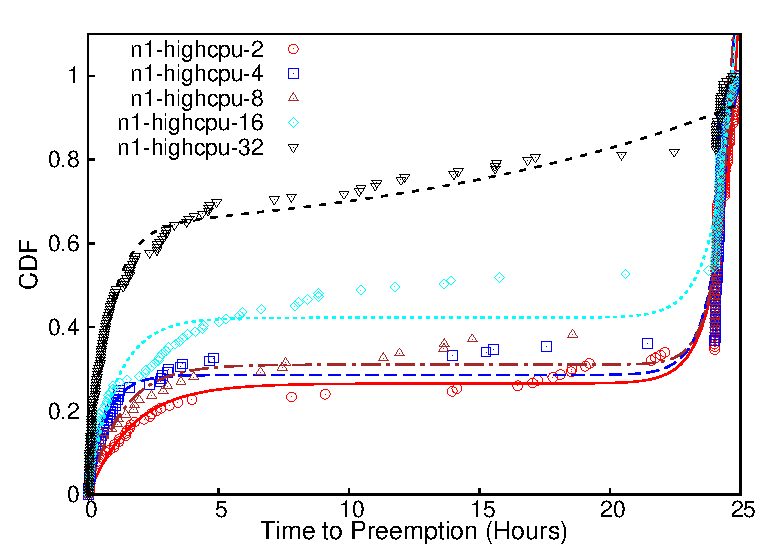
\includegraphics[width=0.4\textwidth]{../graphs/scispot-fig-vm-types.eps}
  \caption{The preemption characteristics of different VM types. Larger VMs are more likely to be preempted.}
  \label{fig:cdf-comparison}
\end{figure}

In general, the preemption dynamics of a VM is determined by the supply and demand of VMs of that \emph{particular} type.
Thus, the preemption characteristics of VMs of different sizes, and running in different geographical zones, are different. 
Figure~\ref{fig:cdf-comparison} shows the preemption data from five different types of VMs in the Google Cloud \texttt{n1-highcpu-\{2,4,8,16,32\}}, where the number indicates the number of CPUs.
All VMs are running in the \texttt{us-central1-c} zone. 
We also show the associated CDFs ($\mathscr{F}$) computed using the proposed model.
% along with the parameters of our four parameter distribution.

From Figure~\ref{fig:cdf-comparison}, we see that the CDFs obtained using our model capture the preemption dynamics of different VM types reasonably well.
For the smallest four VM sizes (2, 4, 8, 16), we find that the initial rate of preemptions ($1/\tau_1 \in [0.5, 1.5]$ $\text{hr}^{-1}$) is typically smaller than the final rate of preemptions ($1/\tau_2 \in [1.28, 1.72]$  $\text{hr}^{-1}$),  and the activation time for the final phase $b \in [24, 24.5]$ hours. 
We note the distinct behavior of the analytical CDF for VMs of size 32, where the fit does not reproduce the final rise accurately but captures the slightly faster increase in preemptions during the middle phase better. 
These plots also illustrate a deficiency in our model, whereby the boundary condition of $\mathscr{F} = 1$ for $t=24$ hours is not strictly imposed.

Interestingly, we can also observe that larger VMs have a higher rate of failure.
This is because larger VMs require more computational resources (such as CPU and memory), and when the supply of resources is low, the cloud operator can reclaim a large amount of resources by preempting larger VMs.
This observed behavior aligns with the guidelines for using preemptible VMs that suggests the use of smaller VMs when possible~\cite{preemptible-documentation}. 

Our analytical model also helps crystallize the differences in VM preemption dynamics, by allowing us to easily calculate their expected lifetime. 
More formally, we define the expected lifetime of a VM of type $i$, as: 
\begin{equation}
  \label{eq:expected-lifetime}
E[L_i] =  \int_{0}^{24} t {p_i}(t)~dt =  -A(t+\tau_1)e^{-t/\tau_1} + A(t-\tau_2) e^{\frac{t-b}{\tau_2}} \biggr\rvert_{0}^{24}
\end{equation}
where $p_i(t)$ is the rate of preemptions of VMs of type $i$ (Equation~\ref{eq:failrate}).
%= \dfrac{d \mathscr{F}(t)} {dt} = A \left(\dfrac{1}{\tau_1}e^{-t/\tau_1} + \dfrac{t-b}{\tau_2}e^{\frac{t-b}{\tau_2}}\right) $ 
%
%Since preemptions require restarting a job and increase the job completion time, it may be more prudent to select transient VMs with higher expected lifetimes.
We use the analytically derived expected lifetimes of VMs of different types in \sysname when selecting the ``best'' VM type for a given bag of jobs. This server selection is a key part of \sysname design, which we describe next. 

% \subsection{EC2 spot instances}

% The earliest form of transient cloud instances.
% In addition to having dynamic availability, also have dynamic pricing.
% ``Classic'' spot instances had price determining the availability, and thus a large amount of work was devoted to bidding and analyzing the prices.

% However a recent change to the spot prices no longer allows these assumptions, rendering it impossible to obtain the \emph{exact} availability information from the prices alone.


% \subsection{Google Preemptible VMs}

% Launched in 2015.
% Flat-rate discount of 80\% compared to on-demand servers.
% Interesting availability SLA: the maximum lifetime is 24 hours, and can be preempted earlier as well.

% In this paper we will look at these preemptible VMs and show how to model their availability.
% Given the inability to use EC2 prices, we believe that our approach is more generalizable and robust.


% There are some distinguishing characteristics of GCP preemptible VMs that makes their failure modeling challenging.
% First is their flat pricing and no other signalling information about their preemption rates (MTBFs) that makes server selection difficult.

% \textbf{Modeling Failure Behavior of Preemptible VMs}
% CDF is ``sigmoid'' shaped.
% $P=R*np.sinh((t-t0)/tau) + C$ with a very low $R=10^{-6}, t_0=12, \tau=0.9, C=0.36$

% Basically, this is a mixture of two distributions, the standard exponential distribution, which we call the stabilization rate and an exponentially increasing reclamation rate.

% Preemptible VMs have three availability phases.

% There are many early deaths, then a period of low failure rates, and then the failure rate is exponential with a positive exponent to enable the cloud provider to reclaim the VMs within the deadline (24 hours in the case of Google's Preemptible VMs).








%%% Local Variables:
%%% mode: latex
%%% TeX-master: "paper"
%%% End:
